\chapter{Описание результатов испытания}
\section{Проведение эксперимента и описание результатов}
Результаты работы алгоритма k-means доступны по следующей ссылке:\linebreak
\url{https://vstu-cad-stuff.github.io/clustering/kmeans/}.

Результаты работы алгоритма k-means со сдвигом центров кластеров к дорожной сети доступны по следующей ссылке:\linebreak
\url{https://vstu-cad-stuff.github.io/clustering/terminals/}.

Для тестирования работы алгоритма было использовано 4 выборки:
\begin{itemize}
    \item выборка \emph{Main}: \( \abs{X} = 12 000 \) точек, \( k = 125 \) (рис.~\ref{pic:full}); используется для общего тестирования работы алгоритмов;
    \item выборка \emph{Railway}: \( \abs{X} = 6 \) точек, \( k = 2 \) (рис.~\ref{pic:railway-river}а); используется для проверки обхода препятствий;
    \item выборка \emph{River}: \( \abs{X} = 6 \) точек, \( k = 2 \) (рис.~\ref{pic:railway-river}б); используется для проверки обхода препятствий;
    \item выборка \emph{Common}: \( \abs{X} = 180 \) точек, \( k = 10 \) (рис.~\ref{pic:common}); используется для тестов алгоритмов на скорость.
\end{itemize}
\begin{figure}[h!]
    \centering
    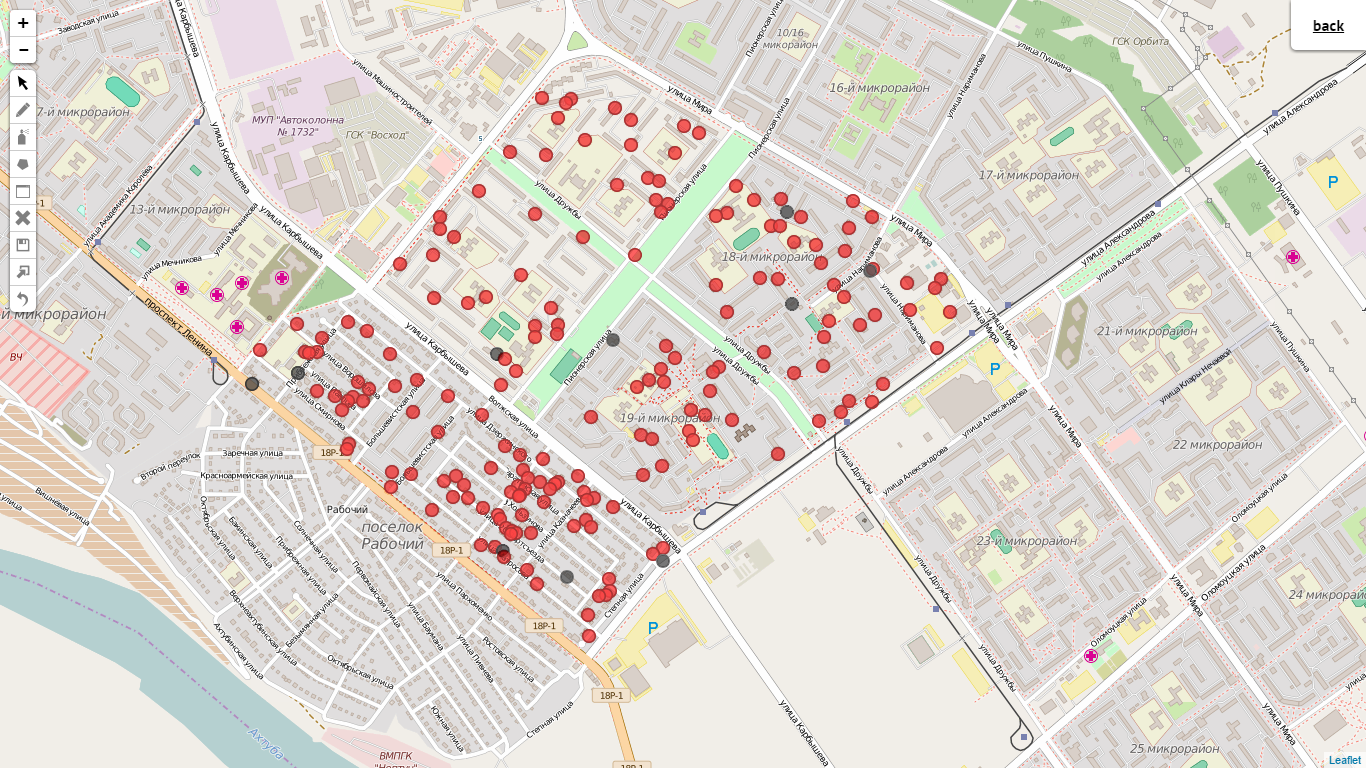
\includegraphics[width=.7\textwidth]{test_common-contrast}\\[1ex]
    \parbox{.9\textwidth}{\caption{Выборка \emph{Common}. Красными кругами отмечены элементы выборки, черными~--- начальные центры кластеров}\label{pic:common}}
\end{figure}

На рисунках, показывающих результаты кластеризации линиями очерчены \emph{кластерные области}~--- выпуклые оболочки множества точек, принадлежащих кластеру.

\subsection{Последовательная реализация}
Данная реализация является наиболее простой из всех с точки зрения расчета расстояния. В данном случае применяется метрика \emph{Surface}. Эта версия может быть интересна в качестве ориентира в тесте на производительность. Данный вариант не позволяет учитывать препятствия, результаты кластеризации выборок \emph{Railway} и \emph{River} представлены на рис.~\ref{pic:test_surface_results}.

\begin{figure}[h!]
    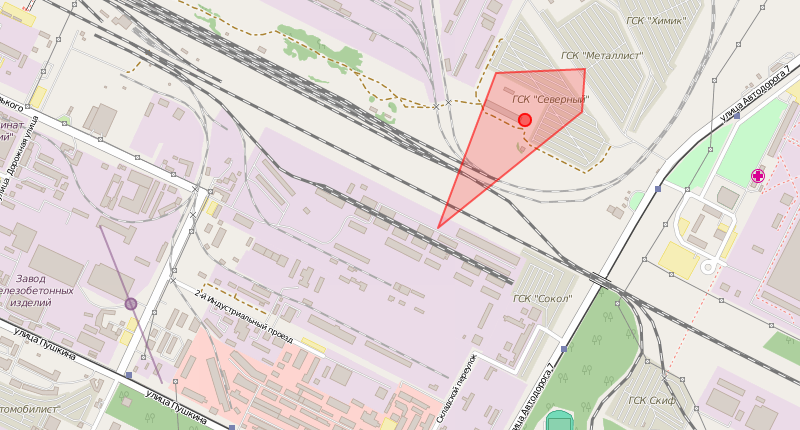
\includegraphics[width=.47\textwidth]{railway_surface}\
    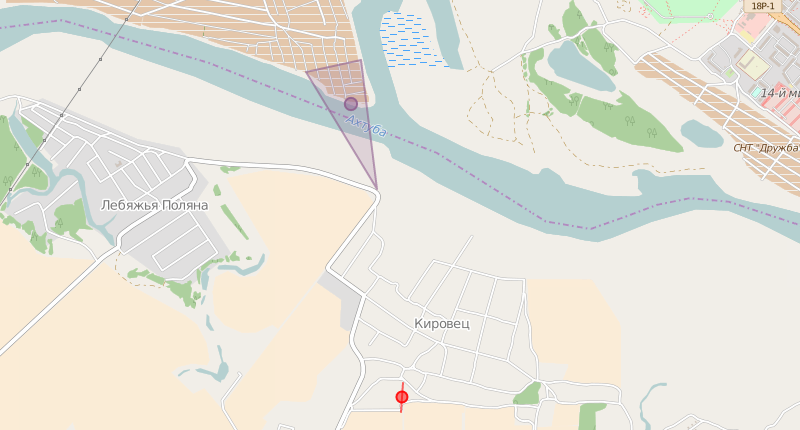
\includegraphics[width=.47\textwidth]{river_surface} \\[1ex]
    \parbox{.95\textwidth}{\caption{Результаты кластеризации выборок \emph{Railway} и \emph{River} с метрикой \emph{Surface}}\label{pic:test_surface_results}}
    \vspace*{-1ex}
\end{figure}

\subsection{Последовательная с использованием OSRM}
Использование метрики \emph{Route} существенно увеличивает время расчета расстояния между объектами. Использование OSRM является узким местом в реализации, однако эта метрика позволяет учитывать препятствия, результаты кластеризации выборок \emph{Railway} и \emph{River} представлены на рис.~\ref{pic:test_route_results}

\begin{figure}[h!]
    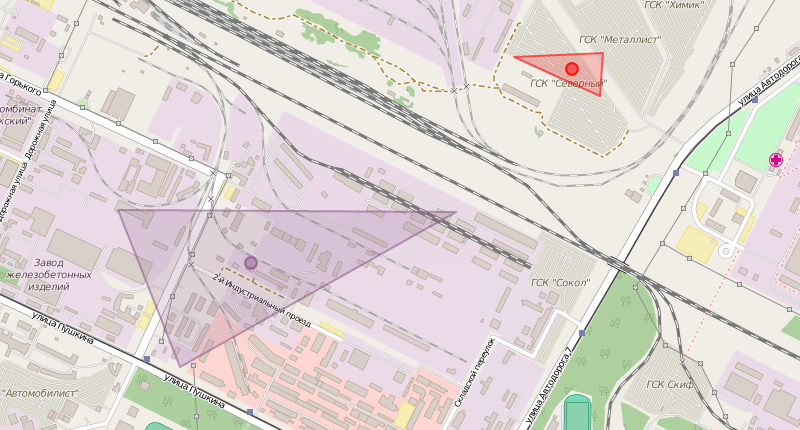
\includegraphics[width=.47\textwidth]{railway_route}\
    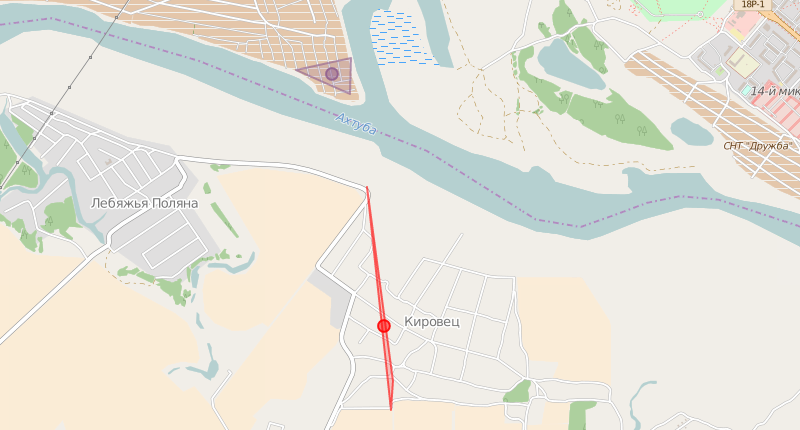
\includegraphics[width=.47\textwidth]{river_route} \\[1ex]
    \parbox{.95\textwidth}{\caption{Результаты кластеризации выборок \emph{Railway} и \emph{River} с метрикой \emph{Route}}\label{pic:test_route_results}}
    \vspace*{-1ex}
\end{figure}

\subsection{Параллельная с использованием OSRM}
Для ускорения расчетов при использовании метрики \emph{Route} предлагается распараллеливание внутреннего цикла по \( X \) (шаги 2.2.1--2.2.4) алгоритма~\ref{alg:kmeans}. Распараллеливание применимо, так как результаты обработки одного объекта выборки не влияют на обработку других объектов.

\subsection{Результаты} \label{sec:workresults}
Результаты обработки выборки \emph{Main} представлены на рисунках~\ref{pic:full-surface}, \ref{pic:full-route}.

\begin{figure}[h!]
    \centering
    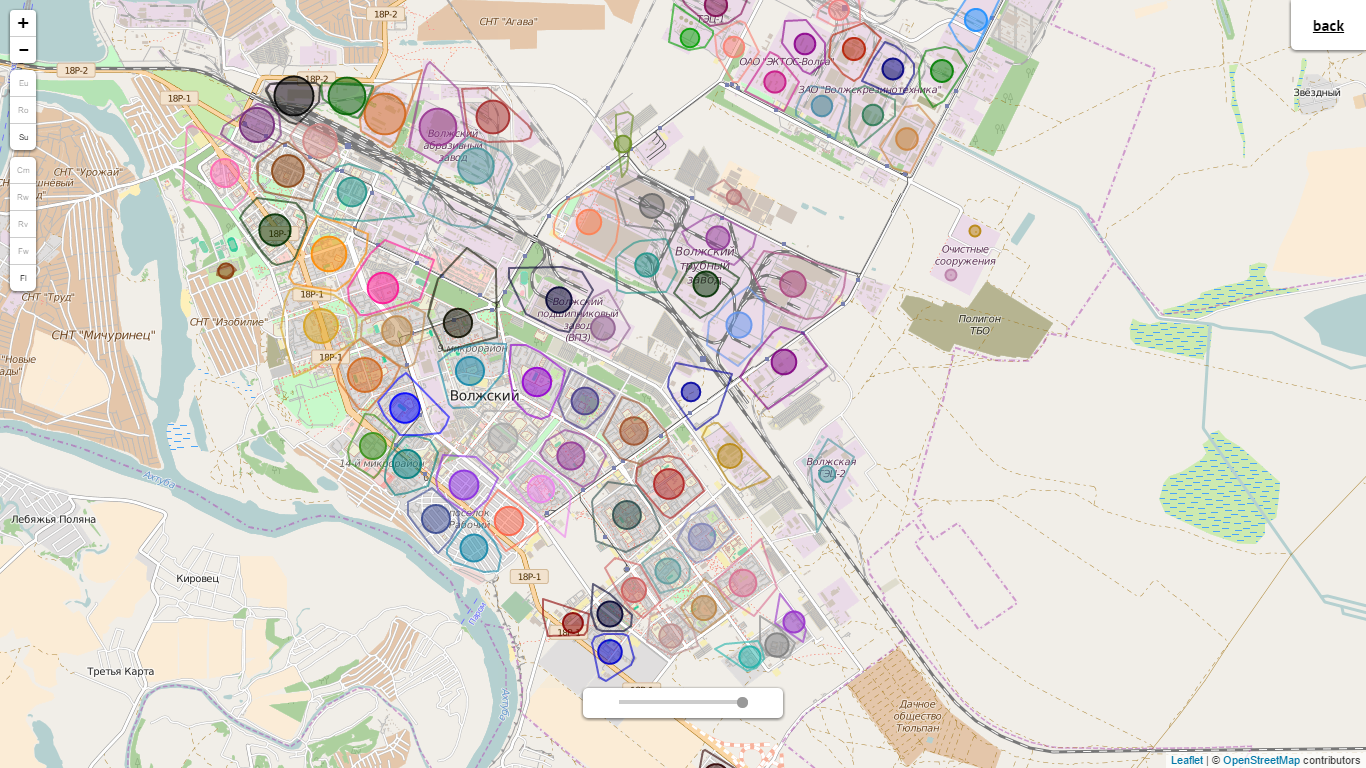
\includegraphics[width=.95\textwidth]{full_surface}\\[1ex]
    \parbox{.95\textwidth}{\caption{Результаты обработки выборки \emph{Main} метрикой \emph{Surface}}\label{pic:full-surface}}
    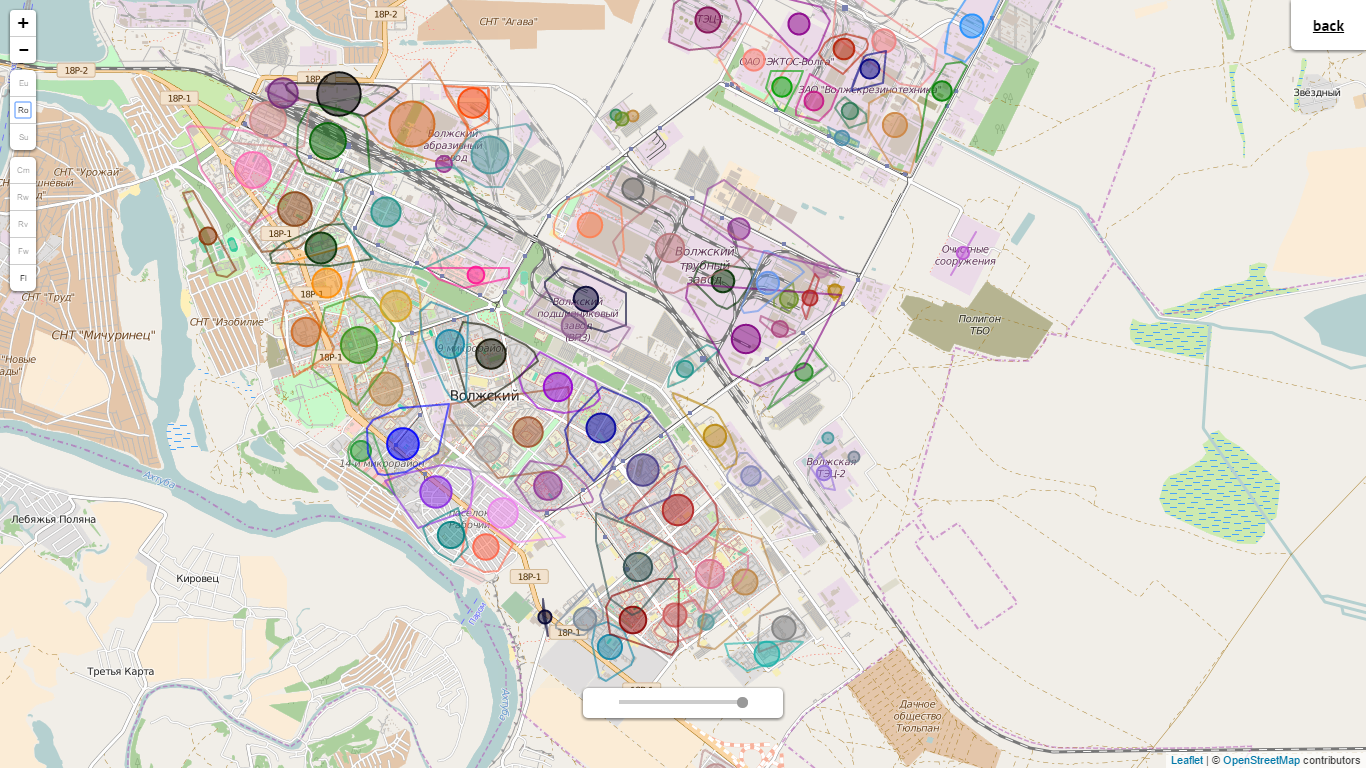
\includegraphics[width=.95\textwidth]{full_route}\\[1ex]
    \parbox{.95\textwidth}{\caption{Результаты обработки выборки \emph{Main} метрикой \emph{Route}}\label{pic:full-route}}
\end{figure}

В таблице~\ref{tab:results} приведены средние длительности выполнения одного расчета дистанции между геопространственными объектами для трех реализаций алгоритма: последовательной, параллельной на два потока и параллельной на 4 потока, и для трех метрик: \emph{Euclid}, \emph{Surface} и \emph{Route}. Метрика \emph{Euclid} является обычной евклидовой метрикой: \( \rho(a, b) = \sqrt{(a.x - b.x)^2 + (a.y - b.y)^2} \) и приводится для сравнения. Величины приведены в миллисекундах.

\begin{table}[h!]
    \centering
    \begin{tabular}{|l|*{3}{C{.15}|}} \hline
        Реализация       & Euclid & Surface & Route \\ \hline
        Последовательная & 0,0665 &  0,709  & 4,785 \\ \hline
        Параллельная (2) & 0,0659 &  0,692  & 4,069 \\ \hline
        Параллельная (4) & 0,0654 &  0,663  & 3,596 \\ \hline
    \end{tabular}
    \caption{Среднее время выполнения одного расчета расстояния при различных метриках и реализациях алгоритма, мс}
    \label{tab:results}
\end{table}

Результат работы алгоритма со сдвигом центров кластеров на ближайший узел графа дорожной сети приведен на рис.~\ref{pic:termmore}:
\begin{figure}[h!]
    \centering
    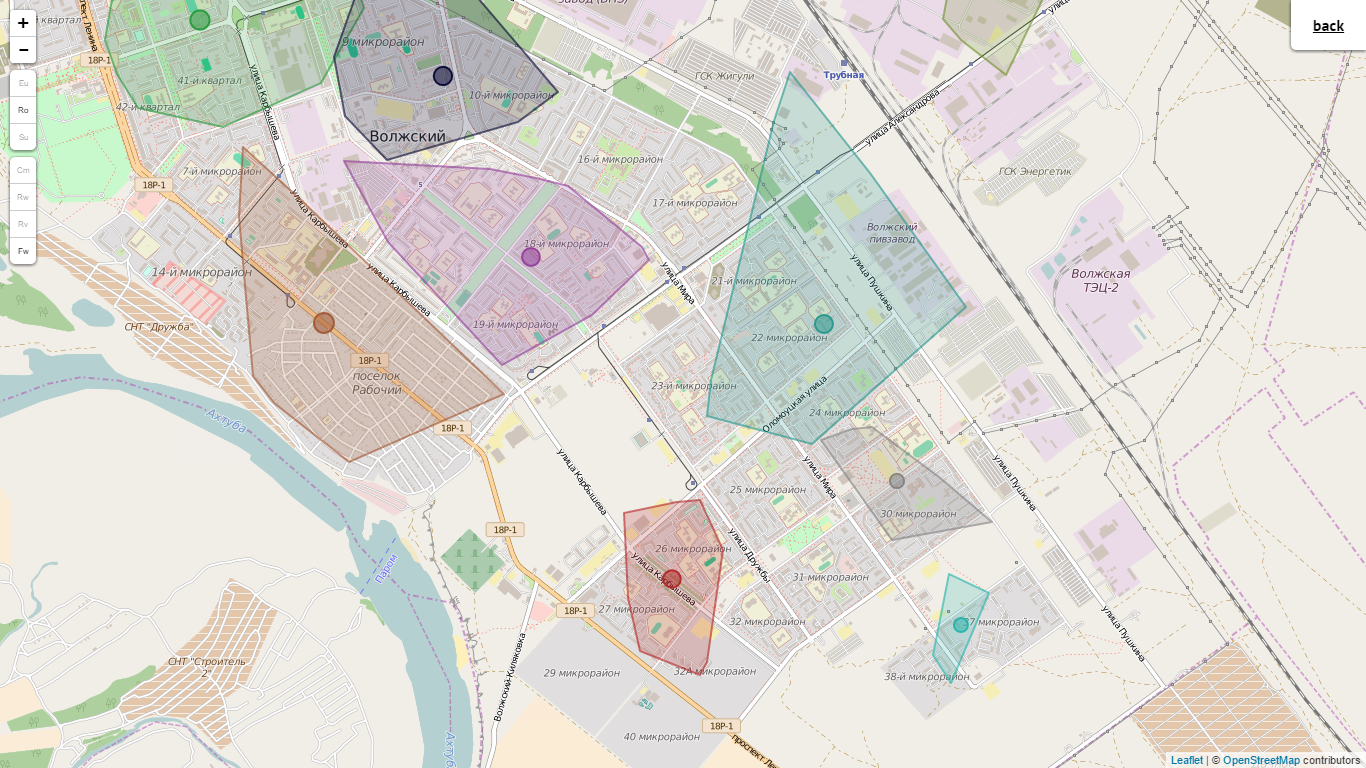
\includegraphics[width=.8\textwidth]{terminals-more}\\[1ex]
    \parbox{.9\textwidth}{\caption{Результат работы алгоритма со сдвигом центров кластеров к дорожной сети}\label{pic:termmore}}
\end{figure}

\section{Обсуждение результатов} \label{sec:preconclusions}
Из рис.~\ref{pic:test_surface_results} видно, что метрика \emph{Surface} не способна учитывать препятствия при расчетах, в то время как метрика \emph{Route} учитывает их (рис.~\ref{pic:test_route_results}). То, что метрика \emph{Surface} не учитывает препятствия, видно и на рисунке~\ref{pic:full-surface}.

На рисунке~\ref{pic:full-route} видно, что кластерные области пересекаются. Это происходит из-за того, что при расчете расстояния сервис OSRM выбирает ближайшие к элементам выборки участки дорожной сети, а затем строит маршрут по графу дорог между ними. Из-за этого элементы, расположенные, например, по разные стороны домов могут попасть на различные участки дорог, и расстояние между ними и центром кластера получается различным. Это также происходит и из-за обхода метрикой препятствий, из-за чего близкие точки оказываются в разных кластерах и создается наложение областей кластеров. Поскольку элементы, принадлежащие одному кластеру, на рисунках показаны в виде выпуклых оболочек, то из-за нескольких элементов кластера, лежащих в стороне от других, создается видимое наложение областей кластеров.

Одна итерация алгоритма при кластеризации выборки \emph{Main} требует \( 12\,000 \times 125 = 1,\!5 \)~млн рассчетов дистанций между объектами выборки и центрами кластеров. При использовании метрики \emph{Surface} кластеризация была выполнена за \( 28 \) итераций алгоритма, то есть потребовалось \( 42 \)~млн расчетов. При использовании метрики \emph{Route} кластеризация была выполнена за \( 21 \) итерацию алгоритма, то есть потребовала \( 31,\!5 \)~млн расчетов расстояний. Таким образом, соотнеся эти сведения с результатами из таблицы~\ref{tab:results}, на одну итерацию с метрикой \emph{Surface} понадобилось примерно \( 16,\!5 \)~минут, на всю кластеризацию~--- около \( 8 \)~часов. На одну итерацию с метрикой \emph{Route} понадобилось примерно \( 1,\!5 \)~часа, а на всю кластеризацию~--- \( 31,\!5 \)~часа или почти полтора дня. Для сравнения, кластеризация с евклидовой метрикой потребовала \( 19 \) итераций, на выполнение которых было потрачено чуть больше получаса. Результат кластеризации выборки \emph{Main} евклидовой метрикой приведен на рис.~\ref{pic:full-euclid}.
\begin{figure}[h!]
    \centering
    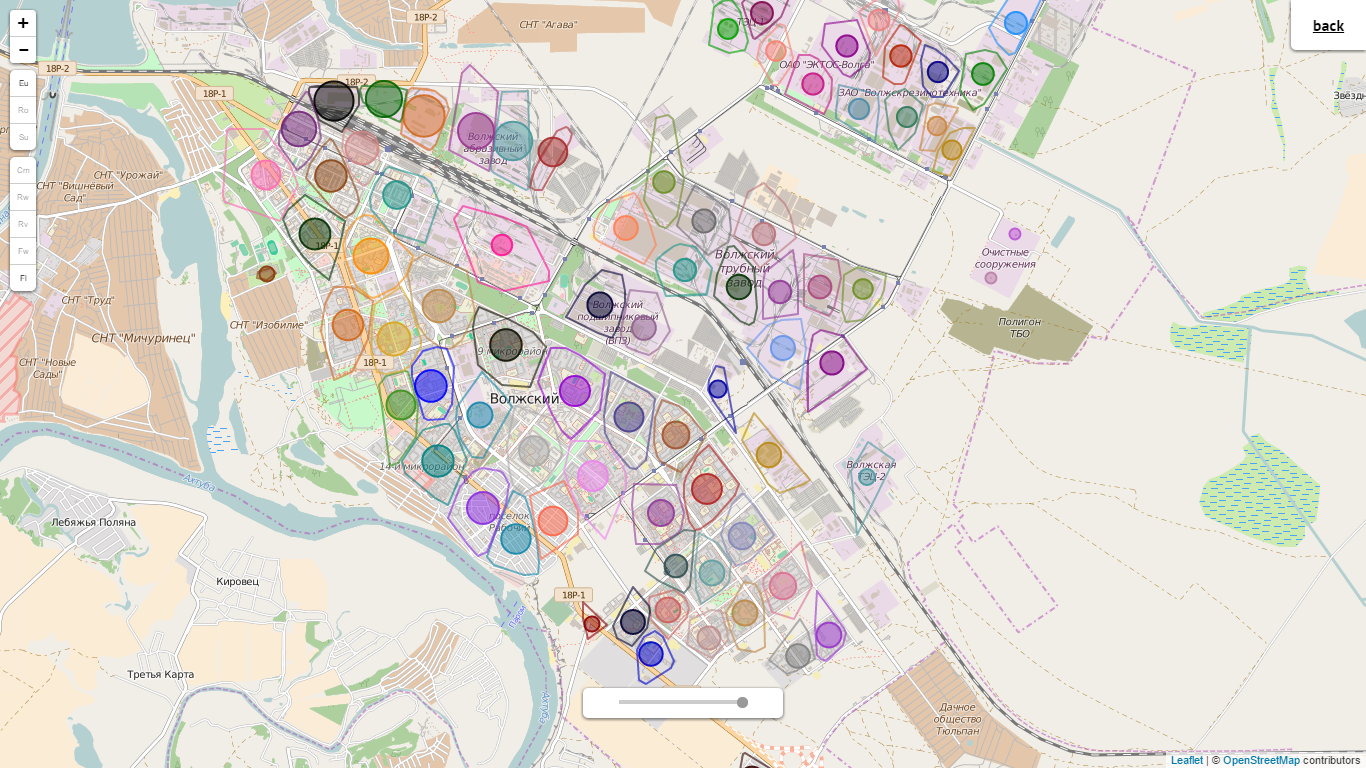
\includegraphics[width=.95\textwidth]{full_euclid} \\[1ex]
    \parbox{.9\textwidth}{\caption{Результаты обработки выборки \emph{Main} евклидовой метрикой}\label{pic:full-euclid}}
    \vspace*{-1em}
\end{figure}

На рисунке~\ref{pic:termmore} видно, что некоторые кластерные центры сдвинулись к магистралям, а некоторые остались в жилых кварталах. Так происходит из-за отсутствия возможности детального рассмотрения кандидатов на расположение центра кластера~--- участков дорожной сети~--- средствами OSRM.

\subsection{Выводы} \label{sec:conclusions}
Подводя итог написанному в предыдущем разделе, можно сказать, что для кластеризации геораспределенных данных предлагаемый подход эффективен по нескольким причинам. Во-первых, ключевой особенностью подхода является использование расстояний между объектами по графу городских дорог позволяет учитывать все препятствия, расположенные между ними. Это позволяет учитывать при кластеризации ситуации, изображенные на рисунке~\ref{pic:2points}. Во-вторых, это также позволяет выполнять основную функцию системы~--- создание остановочных пунктов, расположенных на участках дорог. В-третьих, используется алгоритм k-средних, обладающий невысокой вычислительной сложностью и отсутствием привязки к плотности данных.

Недостатки данного подхода в большей степени связаны со временем, которое требуется сервису OSRM на расчет дистанции. Этот недостаток, вероятно, можно частично сгладить использованием одного из ускоряющих методов из раздела~\ref{sec:methods_}. Также недостатком подхода можно считать определение пользователем числа \( k \) кластеров, однако такой вариант задавания числа кластеров гораздо нагляднее и удобнее для пользователя, чем определение, например, параметра ширины окна в алгоритме Mean Shift. Способом устранить этот недостаток может быть использование предполагающих методов из раздела~\ref{sec:methods_}, например, использование метода силуэтов. Недостаток, связанный с привязкой остановочных пунктов к дорожным узлам внутри жилых кварталов, связан с отсутствием описания точек в ответе сервиса OSRM на запрос. Этот недостаток может быть устранен поиском предложенных OSRM узлов дорожной сети в структруре карты OpenStreetMap, и добавления условия по тэгу (англ. \emph{tag}) с ключом \emph{highway}.

В целом, данный подход может быть использован для кластеризации геораспределенных данных и для построения сети остановочных пунктов общественного транспорта, особенно, если на рассматриваемой местности находятся какие-либо естественные или искусственные препятствия, или время кластеризации не столь важно, как получаемый результат.
